\chapter{学習結果と考察\label{sec:evaluate_estimation_model}}
\thispagestyle{plain}

本章では,第\ref{sec:develop_estimation_model}章で述べた手法で構築した対話雰囲気推定モデルの学習結果と考察について述べる.
はじめに,本研究における対話雰囲気推定モデルの評価手法について述べる.
次に,特徴量選択を用いない対話雰囲気推定モデルの学習結果について述べる.
続いて,特徴量選択を用いた学習の比較基となるベースモデルについて述べる.
最後に,ベースモデルを中心に特徴量選択を用いた学習の結果について述べる.

\section{評価手法}

本研究における対話雰囲気推定モデルの評価はモデル正答率と選択特徴量数を用いる.
これはモデル正答率が高いほど正確な推定が期待でき,選択特徴量数が少ないほど軽量な推定が期待できるためである.
また,モデル評価は第\ref{node:ga}節で述べた個体評価とは異なり,二つの評価観点を一つの評価値と算出することはしない.
これは豊田らの手法においても同様の手法を用いていることと,どちらの観点が重要視されるべきか十分に検討できていないためである.
評価手法の検討については考察で詳細を述べる.

\section{特徴量選択を用いない対話雰囲気推定モデルの学習結果\label{node:learning_result_without_ga}}

対話雰囲気推定モデルの学習における特徴量選択の有効性の評価を行うために,特徴量選択を用いない対話雰囲気推定モデルの構築を行う.
特徴量選択を用いない対話雰囲気推定モデルの学習結果を表\ref{tab:excitement_learning_result_without_FS} 〜 表\ref{tab:comfortable_learning_result_without_FS}に示す.
特徴量選択を用いない対話雰囲気推定モデルは各対象雰囲気,対象話者数,学習モデルを網羅的に組み合わせて構築した.
表中のモデル正答率は有効数字4桁で,小数点第4位を四捨五入したものを掲載している.
いずれにおいても特徴量選択は行なっていないため,学習に利用した特徴量は話者数に依存した最大値となっている.

学習結果から明らかになったことについて述べる.
学習アルゴリズムはいずれの対象雰囲気のモデルにおいても対象話者数が2名または3名の場合,Naive Bayesのモデル正答率が高いことが明らかになった.
一方で,対象話者数が4名のモデルにおけるモデル正答率はモデル番号33の0.300など極端に低い値であるものも確認できる.
また,豊田らの構築した対話雰囲気推定モデルはモデル正答率が0.700 〜 0.855であったことから,これらのモデルのモデル正答率が低いことがわかる.

\begin{table}[ptb]
    \caption{「盛り上がり」を対象とした特徴量選択を用いない学習の結果}
    \centering
    \begin{tabular}{|c|c|l|r|c|}
        \hline
        モデル番号 & 対象話者数 & 学習アルゴリズム & モデル正答率 & 選択特徴量数 \\\hline\hline
        1 & \multirow{4}{*}{2} & Linear SVC & 0.6240 & \multirow{4}{*}{90} \\ \cline{1-1}\cline{3-4}
        2 & & k近傍法 & 0.6400 & \\ \cline{1-1}\cline{3-4}
        3 & & SVC & 0.7040 & \\ \cline{1-1}\cline{3-4}
        4 & & Naive Bayes & 0.7440 & \\ \hline
        5 & \multirow{4}{*}{3} & Linear SVC & 0.4699 & \multirow{4}{*}{144} \\ \cline{1-1}\cline{3-4}
        6 & & k近傍法 & 0.5772 & \\ \cline{1-1}\cline{3-4}
        7 & & SVC & 0.6515 & \\ \cline{1-1}\cline{3-4}
        8 & & Naive Bayes & 0.6632 & \\ \hline
        9 & \multirow{4}{*}{4} & Linear SVC & 0.3300 & \multirow{4}{*}{210} \\ \cline{1-1}\cline{3-4}
        10 & & k近傍法 & 0.5900 & \\ \cline{1-1}\cline{3-4}
        11 & & SVC & 0.6200 & \\ \cline{1-1}\cline{3-4}
        12 & & Naive Bayes & 0.4800 & \\ \hline
    \end{tabular}
    \label{tab:excitement_learning_result_without_FS}
\end{table}

\begin{table}[tpb]
    \caption{「真面目さ」を対象とした特徴量選択を用いない学習の結果}
    \centering
    \begin{tabular}{|c|c|l|r|c|}
        \hline
        モデル番号 & 対象話者数 & 学習アルゴリズム & モデル正答率 & 選択特徴量数 \\\hline\hline
        13 & \multirow{4}{*}{2} & Linear SVC & 0.6362 & \multirow{4}{*}{90} \\ \cline{1-1}\cline{3-4}
        14 & & k近傍法 & 0.4676 & \\ \cline{1-1}\cline{3-4}
        15 & & SVC & 0.5486 & \\ \cline{1-1}\cline{3-4}
        16 & & Naive Bayes & 0.6610 & \\ \hline
        17 & \multirow{4}{*}{3} & Linear SVC & 0.4222 & \multirow{4}{*}{144} \\ \cline{1-1}\cline{3-4}
        18 & & k近傍法 & 0.4417 & \\ \cline{1-1}\cline{3-4}
        19 & & SVC & 0.5583 & \\ \cline{1-1}\cline{3-4}
        20 & & Naive Bayes & 0.6028 & \\ \hline
        21 & \multirow{4}{*}{4} & Linear SVC & 0.5000 & \multirow{4}{*}{210} \\ \cline{1-1}\cline{3-4}
        22 & & k近傍法 & 0.7000 & \\ \cline{1-1}\cline{3-4}
        23 & & SVC & 0.5000 & \\ \cline{1-1}\cline{3-4}
        24 & & Naive Bayes & 0.6000 & \\ \hline
    \end{tabular}
    \label{tab:seriousness_learning_result_without_FS}
\end{table}

\begin{table}[ptb]
    \caption{「明るさ」を対象とした特徴量選択を用いない学習の結果}
    \centering
    \begin{tabular}{|c|c|l|r|c|}
        \hline
        モデル番号 & 対象話者数 & 学習アルゴリズム & モデル正答率 & 選択特徴量数 \\\hline\hline
        25 & \multirow{4}{*}{2} & Linear SVC & 0.5638 & \multirow{4}{*}{90} \\ \cline{1-1}\cline{3-4}
        26 & & k近傍法 & 0.5057 & \\ \cline{1-1}\cline{3-4}
        27 & & SVC & 0.5629 & \\ \cline{1-1}\cline{3-4}
        28 & & Naive Bayes & 0.7181 & \\ \hline
        29 & \multirow{4}{*}{3} & Linear SVC & 0.6722 & \multirow{4}{*}{144} \\ \cline{1-1}\cline{3-4}
        30 & & k近傍法 & 0.5306 & \\ \cline{1-1}\cline{3-4}
        31 & & SVC & 0.5389 & \\ \cline{1-1}\cline{3-4}
        32 & & Naive Bayes & 0.7000 & \\ \hline
        33 & \multirow{4}{*}{4} & Linear SVC & 0.3000 & \multirow{4}{*}{210} \\ \cline{1-1}\cline{3-4}
        34 & & k近傍法 & 0.7000 & \\ \cline{1-1}\cline{3-4}
        35 & & SVC & 0.6000 & \\ \cline{1-1}\cline{3-4}
        36 & & Naive Bayes & 0.4000 & \\ \hline
    \end{tabular}
    \label{tab:cheerfulness_learning_result_without_FS}
\end{table}

\begin{table}[tpb]
    \caption{「くつろぎ」を対象とした特徴量選択を用いない学習の結果}
    \centering
    \begin{tabular}{|c|c|l|r|c|}
        \hline
        モデル番号 & 対象話者数 & 学習アルゴリズム & モデル正答率 & 選択特徴量数 \\\hline\hline
        37 & \multirow{4}{*}{2} & Linear SVC & 0.6200 & \multirow{4}{*}{90} \\ \cline{1-1}\cline{3-4}
        38 & & k近傍法 & 0.5924 & \\ \cline{1-1}\cline{3-4}
        39 & & SVC & 0.5210 & \\ \cline{1-1}\cline{3-4}
        40 & & Naive Bayes & 0.6648 & \\ \hline
        41 & \multirow{4}{*}{3} & Linear SVC & 0.5778 & \multirow{4}{*}{144} \\ \cline{1-1}\cline{3-4}
        42 & & k近傍法 & 0.5806 & \\ \cline{1-1}\cline{3-4}
        43 & & SVC & 0.5583 & \\ \cline{1-1}\cline{3-4}
        44 & & Naive Bayes & 0.7000 & \\ \hline
        45 & \multirow{4}{*}{4} & Linear SVC & 0.6000 & \multirow{4}{*}{210} \\ \cline{1-1}\cline{3-4}
        46 & & k近傍法 & 0.5000 & \\ \cline{1-1}\cline{3-4}
        47 & & SVC & 0.6000 & \\ \cline{1-1}\cline{3-4}
        48 & & Naive Bayes & 0.7000 & \\ \hline
    \end{tabular}
    \label{tab:comfortable_learning_result_without_FS}
\end{table}


\section{ベースモデルの決定\label{node:base_model}}

本研究では,第\ref{node:machine_learning}節と第\ref{node:ga}節で示した各設定値を定めた上で学習を行う.
そこで,特徴選択を行うにあたって各設定値の学習効率への影響を容易に比較するために,比較基となるベースモデルを定める(表\ref{tab:base_model_setting}).
ベースモデルの対象雰囲気は「盛り上がり」とする.
これは豊田らの手法と本研究における推定対象の雰囲気を比較した際に,同一の定義を行っていることに加え,豊田らの研究におけるモデル正答率が0.855と高水準であるためである.
続いて対象話者数は3名とする.
これには二つの理由がある.
一つ目は,豊田らの手法と異なり三者以上の話者を対象とした対話雰囲気推定モデルを構築していることが本研究の独自性の一つであることから,三者以上の話者を対象としたモデルを比較の中心にすることが妥当であると考えたためである.
二つ目は,対象話者数が4名の学習データは第\ref{node:machine_learning}節で述べた前処理を行った結果,学習に用いることができるデータ数が3名に比較し必ず少なくなることから,対象話者数が増加することでモデルの信憑性が低下するためである.
学習アルゴリズムはNaive Bayesを採用する.
これは特徴量選択を行わない学習では,Naive Bayesが最も良いモデル正答率を持っているためである.
それ以降の特徴量選択に関わる設定は,事前に何度か無作為に設定を定めて学習をした上で最もモデル正答率が高く,選択特徴量数が少ないものを採用する.
その際の,評価における重み付け$W$は0.5である.
以上のベースモデルを用いて各学習設定や特徴量選択の有効性を評価する.

\begin{table}[t]
    \caption{ベースモデルの設定値}
    \centering
    \begin{tabular}{ll}
        \hline
        設定項目 & 範囲・候補 \\ \hline\hline
        対象雰囲気 & 盛り上がり \\ \hline
        対象話者数 & 3 \\ \hline
        学習アルゴリズム & Naive Bayes \\ \hline
        交叉方法 & 一様交叉 \\ \hline
        集団の大きさ & 100 \\ \hline
        染色体突然変異率 & 0.05 \\ \hline
        遺伝子突然変異率 & 0.10 \\ \hline
        個体評価方法 & 選択特徴量数とモデル正答率の重み付け和による交差検証 \\ \hline
        選択方法 & エリート選択 \\ \hline
        エリート染色体選択数 & 10 \\ \hline
        世代数 & 250 \\ \hline
    \end{tabular}
    \label{tab:base_model_setting}
\end{table}

\section{特徴量選択を用いた対話雰囲気推定モデルの学習結果\label{node:learning_result_with_ga}}

第\ref{node:base_model}節で述べたベースモデルを基に特徴量選択を用いた対話雰囲気推定モデルを構築する.
はじめに,ベースモデルから対象雰囲気,話者数を変更したモデルについて述べ,続いて特徴量選択の各設定を変更したモデルについて述べる.

\subsection{対象雰囲気,話者数を変更したモデルの学習結果\label{item:learning_result_with_ga_change_targets}}

ベースモデルとベースモデルから対象雰囲気,話者数を変更した全てのモデルの学習結果の一例を表\ref{tab:learn_result_with_ga}に示す.
表中のモデル番号50がベースモデルを表している.

\begin{table}[t]
    \caption{特徴量選択を用いたモデルの学習結果}
    \centering
    \begin{tabular}{|c|c|c|r|r|}
        \hline
        モデル番号 & 対象雰囲気 & 対象話者数 & モデル正答率 & 選択特徴量数 \\
        \hline\hline
        49 & \multirow{3}{*}{盛り上がり} & 2 & 0.800 & 10 \\ \cline{1-1}\cline{3-5}
        50 & & 3 & 0.795 & 21 \\ \cline{1-1}\cline{3-5}
        51 & & 4 & 0.860 & 45 \\ \hline
        52 & \multirow{3}{*}{真面目さ} & 2 & 0.775 & 16 \\ \cline{1-1}\cline{3-5}
        53 & & 3 & 0.769 & 30 \\ \cline{1-1}\cline{3-5}
        54 & & 4 & 0.800 & 38 \\ \hline
        55 & \multirow{3}{*}{明るさ} & 2 & 0.830 & 12 \\ \cline{1-1}\cline{3-5}
        56 & & 3 & 0.863 & 33 \\ \cline{1-1}\cline{3-5}
        57 & & 4 & 0.700 & 40 \\ \hline
        58 & \multirow{3}{*}{くつろぎ} & 2 & 0.790 & 13 \\ \cline{1-1}\cline{3-5}
        59 & & 3 & 0.816 & 25 \\ \cline{1-1}\cline{3-5}
        60 & & 4 & 0.900 & 40 \\ \hline
    \end{tabular}
    \label{tab:learn_result_with_ga}
\end{table}

この結果から明らかになったことについて述べる.

はじめに,ベースモデルに着目する.
特徴量選択を行う前のベースモデルと同条件のモデルは表\ref{tab:excitement_learning_result_without_FS}のモデル番号8である.
これらのモデルを比較するとモデル正答率が0.663から0.795に向上し,選択特徴量数が144から21に減少していることが確認できる.
ベースモデルの学習過程を図\ref{fig:exc3_crossover}に示す.
図\ref{fig:exc3_crossover}は横軸がGAの世代数を表しており,オレンジ色の値がモデル正答率,緑色の値が全体に対する選択特徴量数の割合,青色が評価値を表している.
図\ref{fig:exc3_crossover}からも学習が進むにつれてモデル正答率と選択特徴量数が変化していることがわかる.

\begin{figure}
    \centering
    \fbox{
        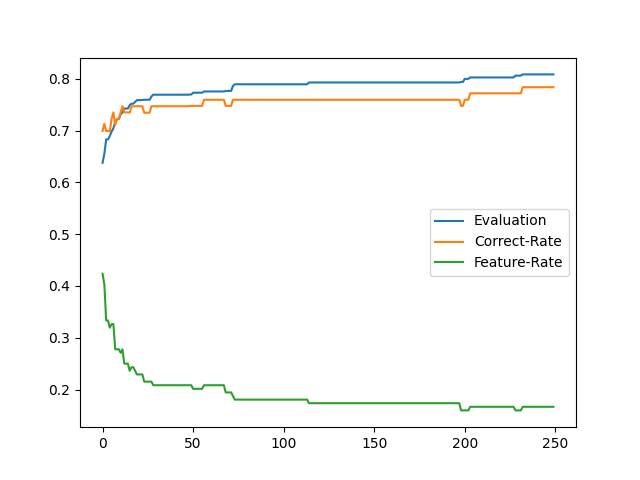
\includegraphics[width=0.7\textwidth]{figs/exc3_crossover.png}
    }
    \caption{ベースモデルの学習過程}
    \label{fig:exc3_crossover}
\end{figure}

次に,全体のモデル正答率に着目する.
ベースモデル同様,全体としてモデル正答率の向上を確認できる.
事実,表\ref{tab:excitement_learning_result_without_FS} 〜 表\ref{tab:comfortable_learning_result_without_FS}のうちNaive Bayesを学習モデルとして採用しているモデルと,表\ref{tab:learn_result_with_ga}のモデルのモデル正答率について両側5%のt検定を行った結果,P値が$3.5727 \times 10^{-5}$を示すことから有意差を確認できる(表\ref{tab:correct_rate_t-test}).
豊田らの構築した対話雰囲気推定モデルの正答率と比較しても大きな差は見られず同程度の精度を持つモデルであることがわかる.
また,対象雰囲気間によるモデル正答率の差は小さいことが確認できる.
一方で,話者数の増加に伴ってモデル正答率が不安定になっていることが確認できる.
特に,対象話者が4名の場合は顕著である(図\ref{fig:exc4} 〜 図\ref{fig:com4}).

\begin{table}[t]
    \caption{特徴量選択前後のモデル正答率のt検定}
    \centering
    \begin{tabular}{cc}
        \hline
        算出項目 & 算出値 \\
        \hline\hline
        \multirow{2}{*}{平均値} & 特徴量選択前: $0.6362$ \\
        & 特徴量選択後: $0.8085$ \\ \hline
        \multirow{2}{*}{分散値} & 特徴量選択前: $0.0105$ \\
        & 特徴量選択後: $0.0027$ \\ \hline
        t値 & $-6.6579$ \\ \hline
        t境界値 & $2.2010$ \\ \hline
        P値 & $3.5727 \times 10^{-5}$ \\ \hline
    \end{tabular}
    \label{tab:correct_rate_t-test}
\end{table}

\begin{figure}
    \centering
    \fbox{
        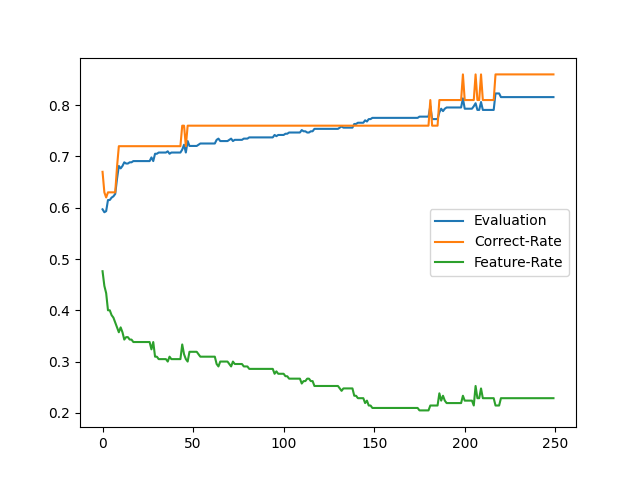
\includegraphics[width=0.7\textwidth]{figs/exc4.png}
    }
    \caption{「盛り上がり」話者数4名のモデル学習過程}
    \label{fig:exc4}
\end{figure}

\begin{figure}
    \centering
    \fbox{
        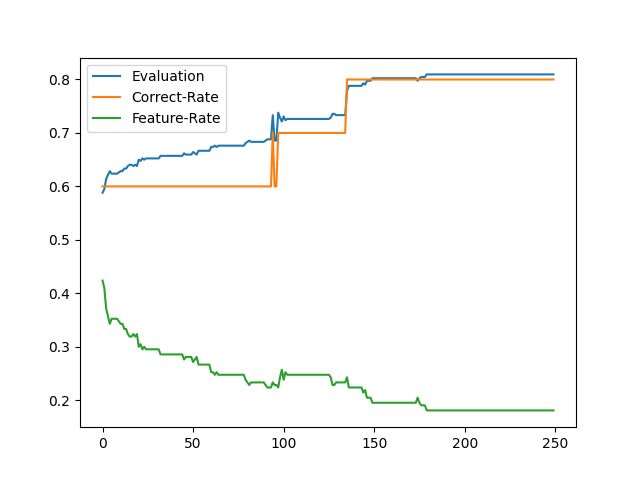
\includegraphics[width=0.7\textwidth]{figs/ser4.png}
    }
    \caption{「真面目さ」話者数4名のモデル学習過程}
    \label{fig:ser4}
\end{figure}

\begin{figure}
    \centering
    \fbox{
        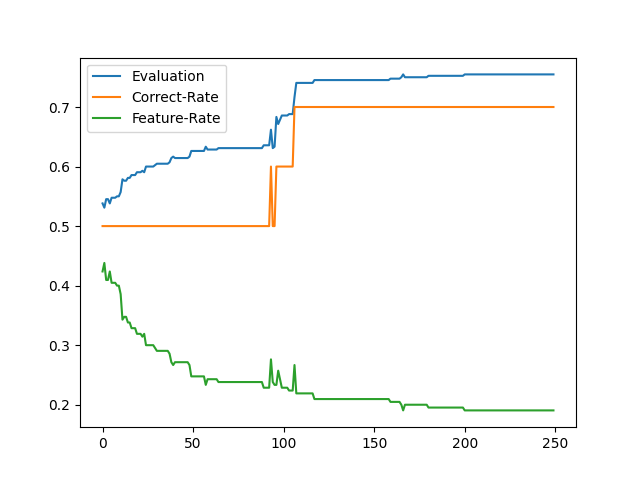
\includegraphics[width=0.7\textwidth]{figs/che4.png}
    }
    \caption{「明るさ」話者数4名のモデル学習過程}
    \label{fig:che4}
\end{figure}

\begin{figure}
    \centering
    \fbox{
        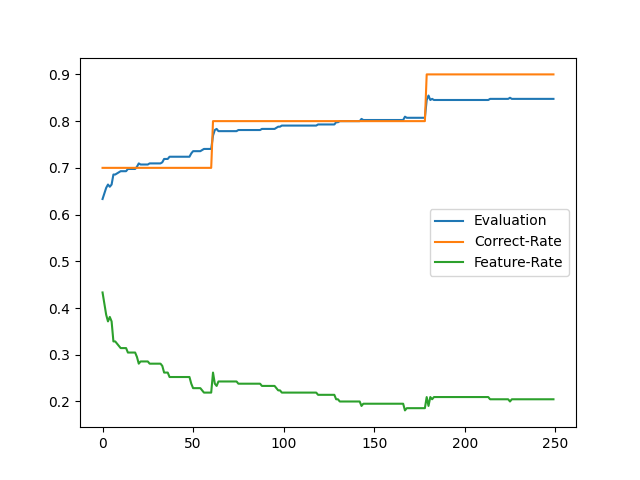
\includegraphics[width=0.7\textwidth]{figs/com4.png}
    }
    \caption{「くつろぎ」話者数4名のモデル学習過程}
    \label{fig:com4}
\end{figure}

最後に選択特徴量数に着目する.
全ての対象雰囲気において対象話者数の増加に伴って,選択特徴量数の増加を確認できる.
一方で,同じ対象話者数のモデルを対象雰囲気間で比較しても大きな差は確認できない.
また,選択特徴量数とモデル正答率においても本結果からは相関を確認することはできない.

\subsection{特徴量選択の設定を変更したモデルの学習結果\label{item:learning_result_with_ga_change_params}}

ベースモデから特徴量選択の各設定を変更した対話雰囲気推定モデルの学習結果の一部を表\ref{tab:learn_result_with_ga_change_params}に示す.
表中の各モデルについて変更点と得られた学習結果について述べる.

モデル番号61は評価における交差検証を排除したモデルである.
表中に掲載しているものはベースモデルと比較して高いモデル正答率を示しているが,何度か同条件でモデルを構築した際には0.6前後のモデル正答率を示す場合も確認できた.

モデル番号62 〜 64は個体評価における重み付けを変更したモデルである.
ベースモデルは重み付け$W$は0.5に設定している.
表中のモデルの$W$は,それぞれモデル番号62は1.0,モデル番号63は0.9,モデル番号64は0.1に設定している.
ベースモデルと各モデルを比較すると,$W$が小さくなるに従って選択特徴量数が減少することがわかる.
一方で,$W$を大きくしてもモデル正答率に大きな影響がないことが確認できる.

モデル番号65は交叉方法を変更し,二点交叉を採用したモデルである.
ベースモデルと比較すると,モデル正答率の僅かな減少と選択特徴量数の僅かな増加が確認できる.
これらの状況は交叉方法だけでなく,突然変異率や集団の大きさなどを変更した際にも同様の結果が得られる.

モデル番号66 〜 68は学習アルゴリズムを変更したモデルである.
Linear SVCとk近傍法を採用したモデルは,特徴量選択を用いないモデルと同様のモデル正答率が確認できる.
また,ベースモデルと比較するとモデル正答率の減少,選択特徴量数の増加が確認できる.
SVCを採用したモデルはベースモデルと同様の学習結果であることが確認できる.

\begin{table}[t]
    \caption{特徴量選択を用いたモデルの学習結果}
    \centering
    \begin{tabular}{|c|c|r|r|}
        \hline
        モデル番号 & モデル概要 & モデル正答率 & 選択特徴量数 \\
        \hline\hline
        50 & ベースモデル(再掲載) & 0.795 & 21 \\ \hline
        61 & 交差検証なしモデル & 0.833 & 21 \\ \hline
        62 & $W:1.0$モデル & 0.796 & 62 \\ \hline
        63 & $W:0.9$モデル & 0.786 & 42 \\ \hline
        64 & $W:0.1$モデル & 0.688 & 14 \\ \hline
        65 & 二点交叉モデル & 0.783 & 24 \\ \hline
        66 & Linear SVCモデル & 0.711 & 28 \\ \hline
        67 & k近傍法モデル & 0.710 & 18 \\ \hline
        68 & SVCモデル & 0.802 & 19 \\ \hline
    \end{tabular}
    \label{tab:learn_result_with_ga_change_params}
\end{table}

\section{学習結果の考察}

第\ref{node:learning_result_without_ga}節,第\ref{node:learning_result_with_ga}節で述べた学習結果に対する考察について述べる.

はじめに,特徴量選択の有用性について述べる.
本研究では,特徴量選択を用いない対話雰囲気推定モデルと用いた対話雰囲気推定モデルをそれぞれ構築している.
それぞれの比較を行なった結果,多くのモデルでモデル正答率の向上と選択特徴量数の減少を確認できる.
このことから,本研究で構築する対話雰囲気推定モデルにおいても特徴量選択が有効であるといえる.
特徴量選択の最適な設定については,第\ref{item:learning_result_with_ga_change_params}項で示した結果などからベースモデルが最適であることが示唆された.
個体評価においては,重み付け和を採用することの有用性は示唆されているものの,最適な重み付け$W$を一意に定めることはできなかった.
これは,GAを採用していることから学習の過程で乱数が発生し,それにより結果が変動するためである.
よって,今後の課題として乱数を加味した上で最適な個体評価を行う手法の検討が挙げられる.
しかし,本研究で構築したベースモデルは正答率,選択特徴量数ともに十分な値であることから,本研究では$W$は0.5を現状の最適値とし採用する.

次に,話者数の増加に伴う選択特徴量数の増加とモデル正答率の不安定化について述べる.
第\ref{item:learning_result_with_ga_change_targets}項で述べた通り,モデルの対象話者数の増加により選択特徴量数が増加している.
一般に選択特徴量数は少ない方が望ましく,豊田らの手法では2 〜 5個にまで選択数を削減している.
しかし,本研究では第\ref{node:pickup_feature}節で述べた通り最大210個の特徴量を抽出しており,母数からの削減割合でみると大きぐ削減に成功していることがわかる.
また,話者数の増加に伴う選択特徴量数の増加についても,話者数が増えるに従って母数となる選択特徴量が多くなるためである.
したがって,話者数の増加に伴う選択特徴量数の増加についてはモデルの評価へは影響が少ないと考えられる.
一方で,話者数の増加に伴ってモデル正答率が不安定になっている現象への解決は大きな課題である.
この問題の原因は学習データが少ないことにある.
本研究のモデル構築手法は学習を行う直前に前処理として,対象話者数に依存した欠損値を含む学習データの削減を行なっている.
それに伴い,話者数が増加するに従って学習データが不足し,結果としてモデル正答率が不安定になっている.
よって,原因の解決としては学習データの拡充が挙げられる.
しかし,本研究における学習データの収集,構築方法は複雑であり,一つの学習データを作成するために30分以上の時間を有する場合もある.
そこで,学習データの自動収集システムを構築することが解決手段の一つとして挙げられる.
具体的には,人間の主観による判断が必要のない全ての作業をシステムに代替し,主観による判断が問われる学習データへのラベル付けだけを行うシステムを構築することで問題の解決が期待できる.

しかし,学習データを自動で収集するシステムの構築には対話の検知を行わなくてはいけないという課題がある.
第\ref{node:deta_collection}節で述べた手法のうち,対話データの切り分けは人間の主観によって話題を判断し,その切り替わりと同時に切り分けを行なっている.
システムによって,自動化を行う際には話題の切り替わりをシステムによって判断する必要がある.
また,第\ref{item:estimation_module_collection_data}項で述べた通り本研究では参加者のプライバシーの担保と,学習コストの低減を目的に言語情報の収集を行わない.
つまり,非言語情報である発話時間情報のみを用いて話題の切り替わりを判断する必要がある.
その方法として対話中の無音時間による検知を提案する.
話題の切り替わり時には誰も喋らず無音の時間が発生することが多い.
特に0.5 〜 2秒程度の無音時間が続いた場合には話題の切り替わりが頻繁に発生していた.
また,話題の切り替わりが発生した際に途端に対話雰囲気が変化することは稀であり,対話雰囲気は自然に移行する性質も確認できている.
よって,厳密な話題の切り替わりを判断する必要性は薄く,本手法で十分に対応が可能であるといえる.
また,収集した学習データのうち無作為に抽出したいくつかを対話雰囲気推定結果とともにユーザへ示し,ユーザが修正できるような仕組みを導入することで適切な学習データの収集やモデル構築が期待できる.
